%% ============================================================
%%  SECCIÓN 10 — Gráficas
%% ============================================================

\section{Gráficas}
\label{sec:graficas}

En esta sección se presentan las representaciones gráficas científicas generadas a partir de los datos experimentales recolectados en el laboratorio. Las figuras fueron procesadas y renderizadas a alta resolución (\qty{300}{DPI}) mediante un script modular en Python~\cite{script_graficas} empleando las librerías científicas \texttt{NumPy}~\cite{numpy}, \texttt{SciPy}~\cite{scipy} y \texttt{Matplotlib}~\cite{matplotlib}, incorporando barras de error bidireccionales ($\pm \delta V, \pm \delta I$), formateadores de coma decimal y paneles de residuos para evaluar la bondad de los modelos ajustados.

\subsection{Curva Característica de la Resistencia de Carbón (Ley de Ohm)}
En la Figura~\ref{fig:grafica_resistencia_ohmica} se presenta la característica $I$ vs $V$ para la resistencia de composición de carbón de valor nominal \qty{100}{\ohm}, junto con la recta de ajuste por mínimos cuadrados ordinarios (MCO), la respuesta teórica ideal y el panel inferior de residuos.

\begin{figure}[H]
    \centering
    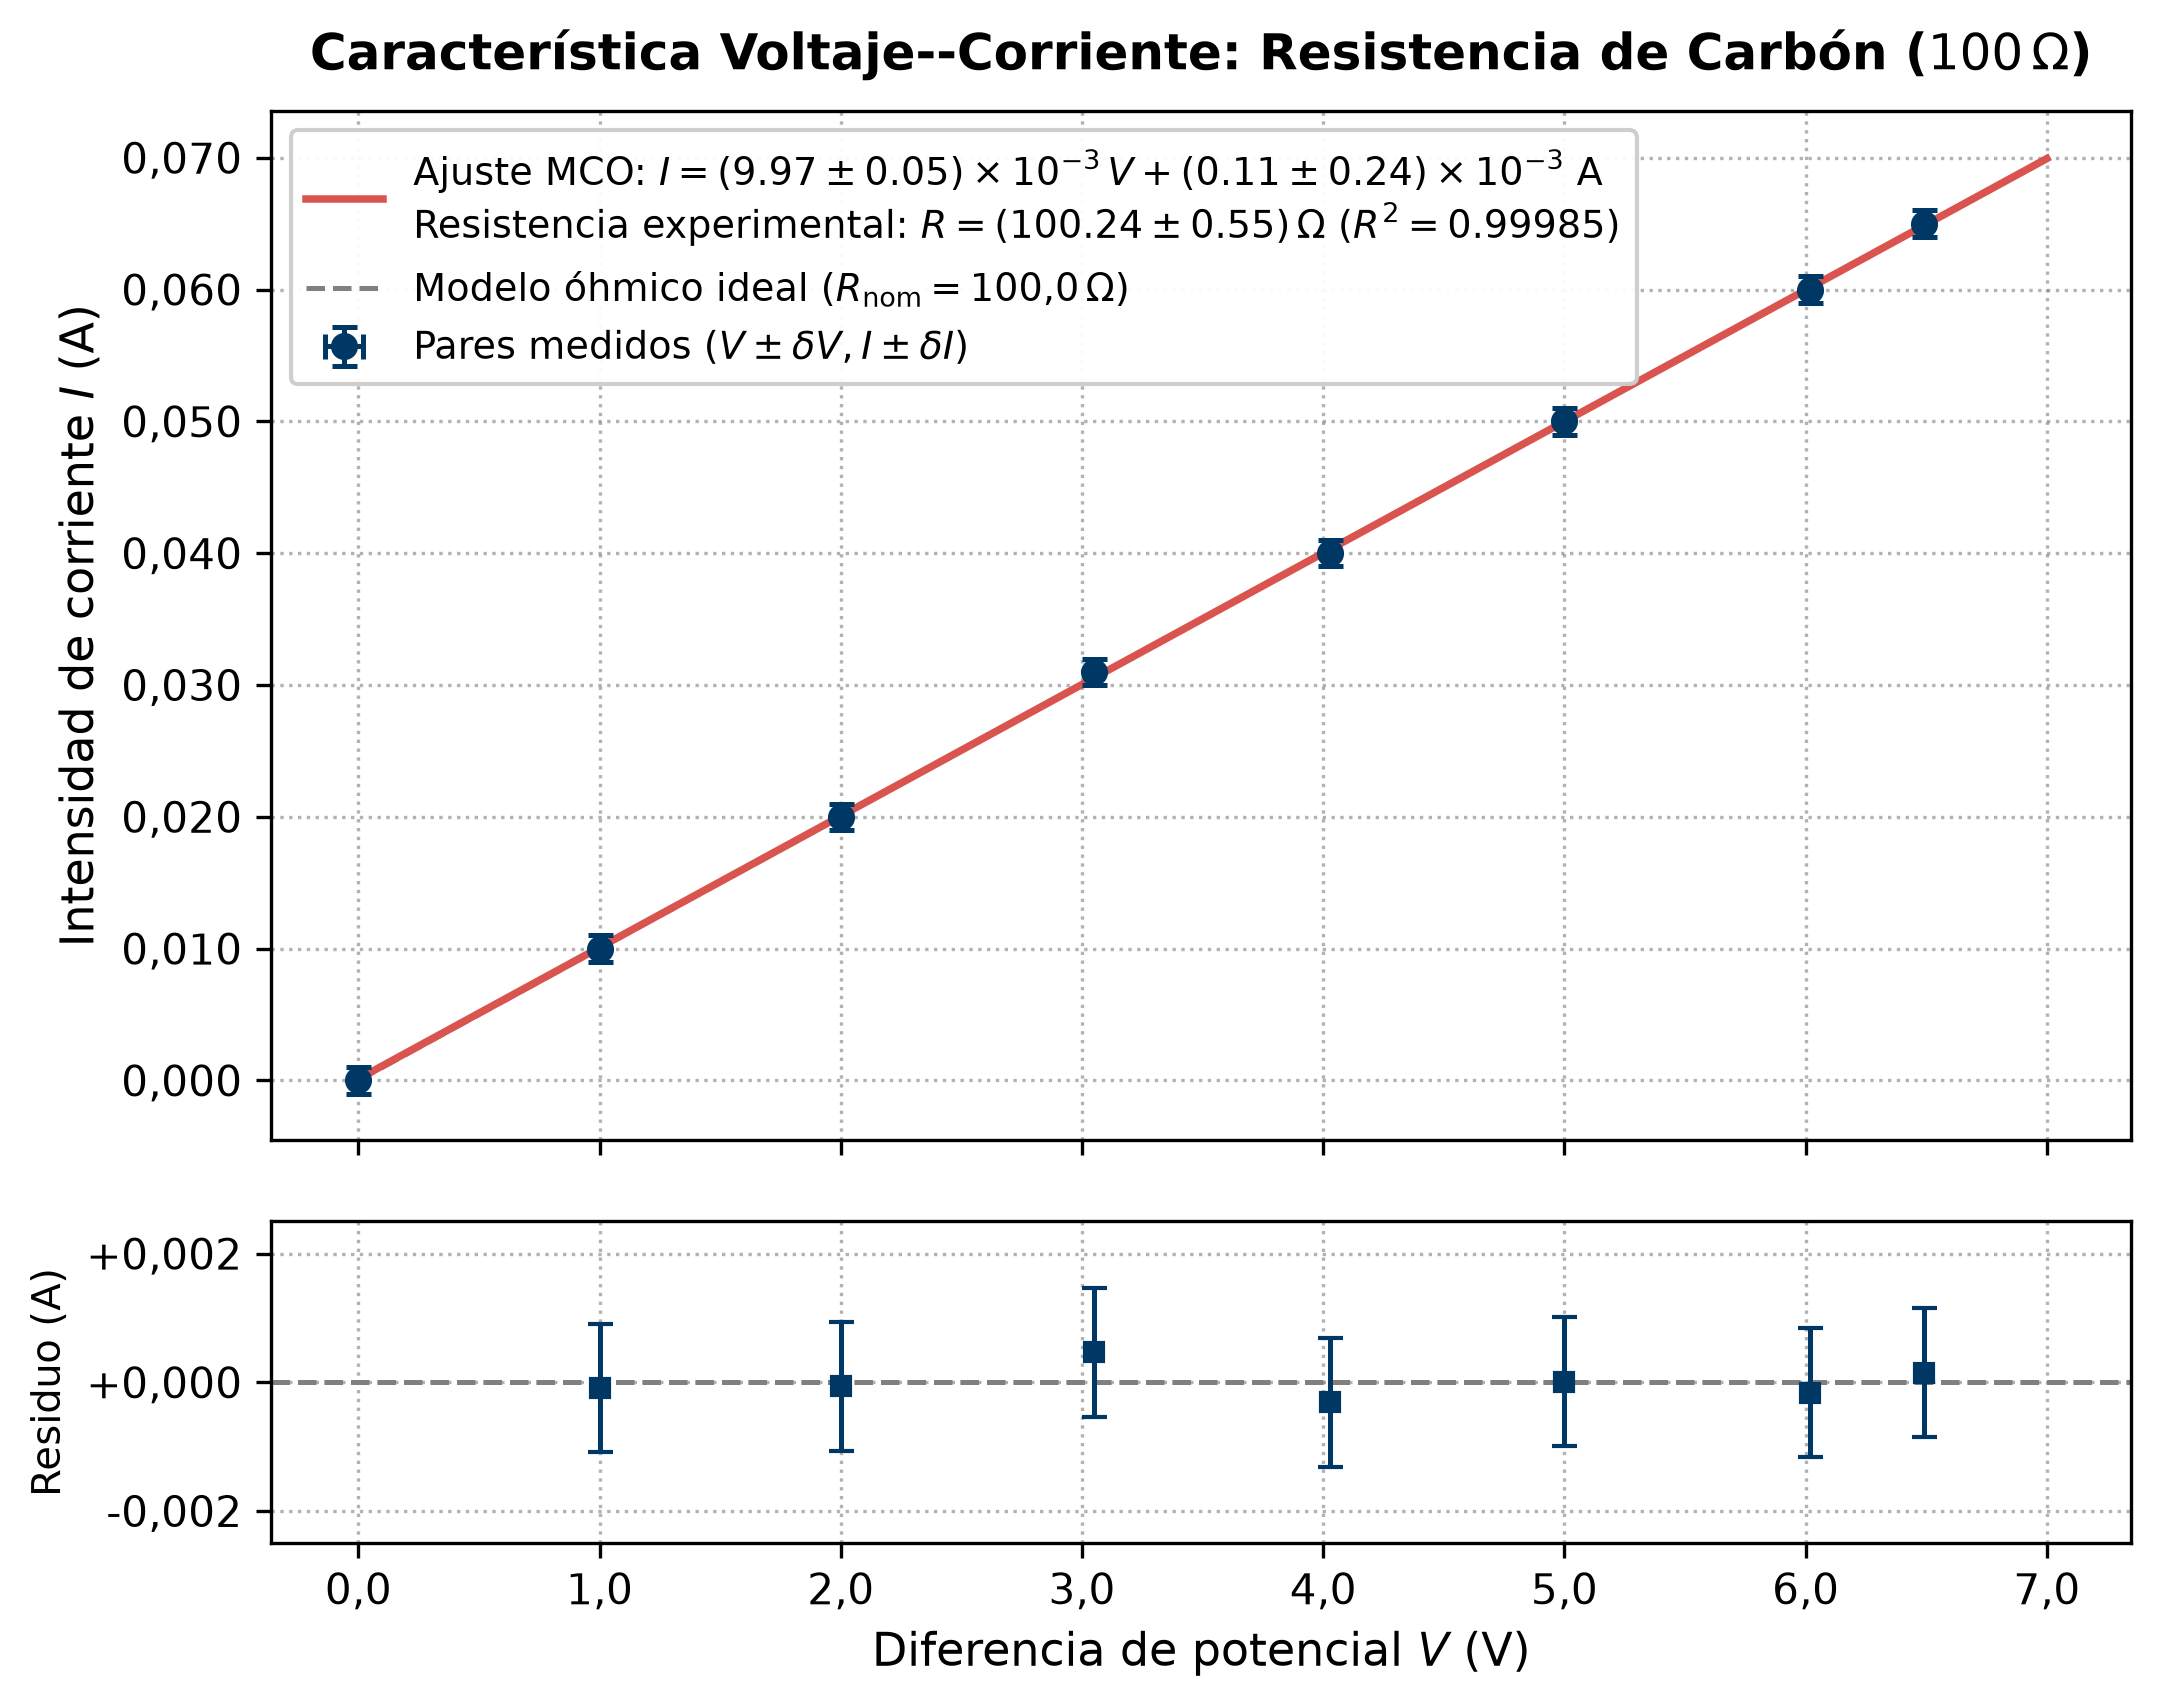
\includegraphics[width=0.85\linewidth]{fig_resistencia_ohmica}
    \caption{Curva característica $I$ vs $V$ de la resistencia de carbón de \qty{100}{\ohm}. Los puntos azules representan los datos experimentales con barras de error ($\pm\qty{0,01}{\volt}, \pm\qty{0,001}{\ampere}$). La línea continua roja muestra el ajuste por MCO ($R = \qty{100,25 \pm 0,55}{\ohm}, R^2 = 0{,}99985$) y la línea discontinua gris representa el modelo ideal ($R_{\text{nom}} = \qty{100,0}{\ohm}$). El panel inferior expone los residuos del ajuste contenidos en $\pm\qty{1}{\milli\ampere}$. Gráfica generada mediante script en Python~\cite{script_graficas}.}
    \label{fig:grafica_resistencia_ohmica}
\end{figure}

\subsection{Curva Característica de la Lámpara Incandescente (Filamento de Tungsteno)}
En la Figura~\ref{fig:grafica_foquito_tungsteno} se ilustra el comportamiento de la lámpara incandescente de tungsteno, contrastando los puntos experimentales frente al modelo no lineal de ley de potencias $I = k V^n$ derivado del balance térmico de Stefan-Boltzmann, incluyendo la tangente en frío y los residuos.

\begin{figure}[H]
    \centering
    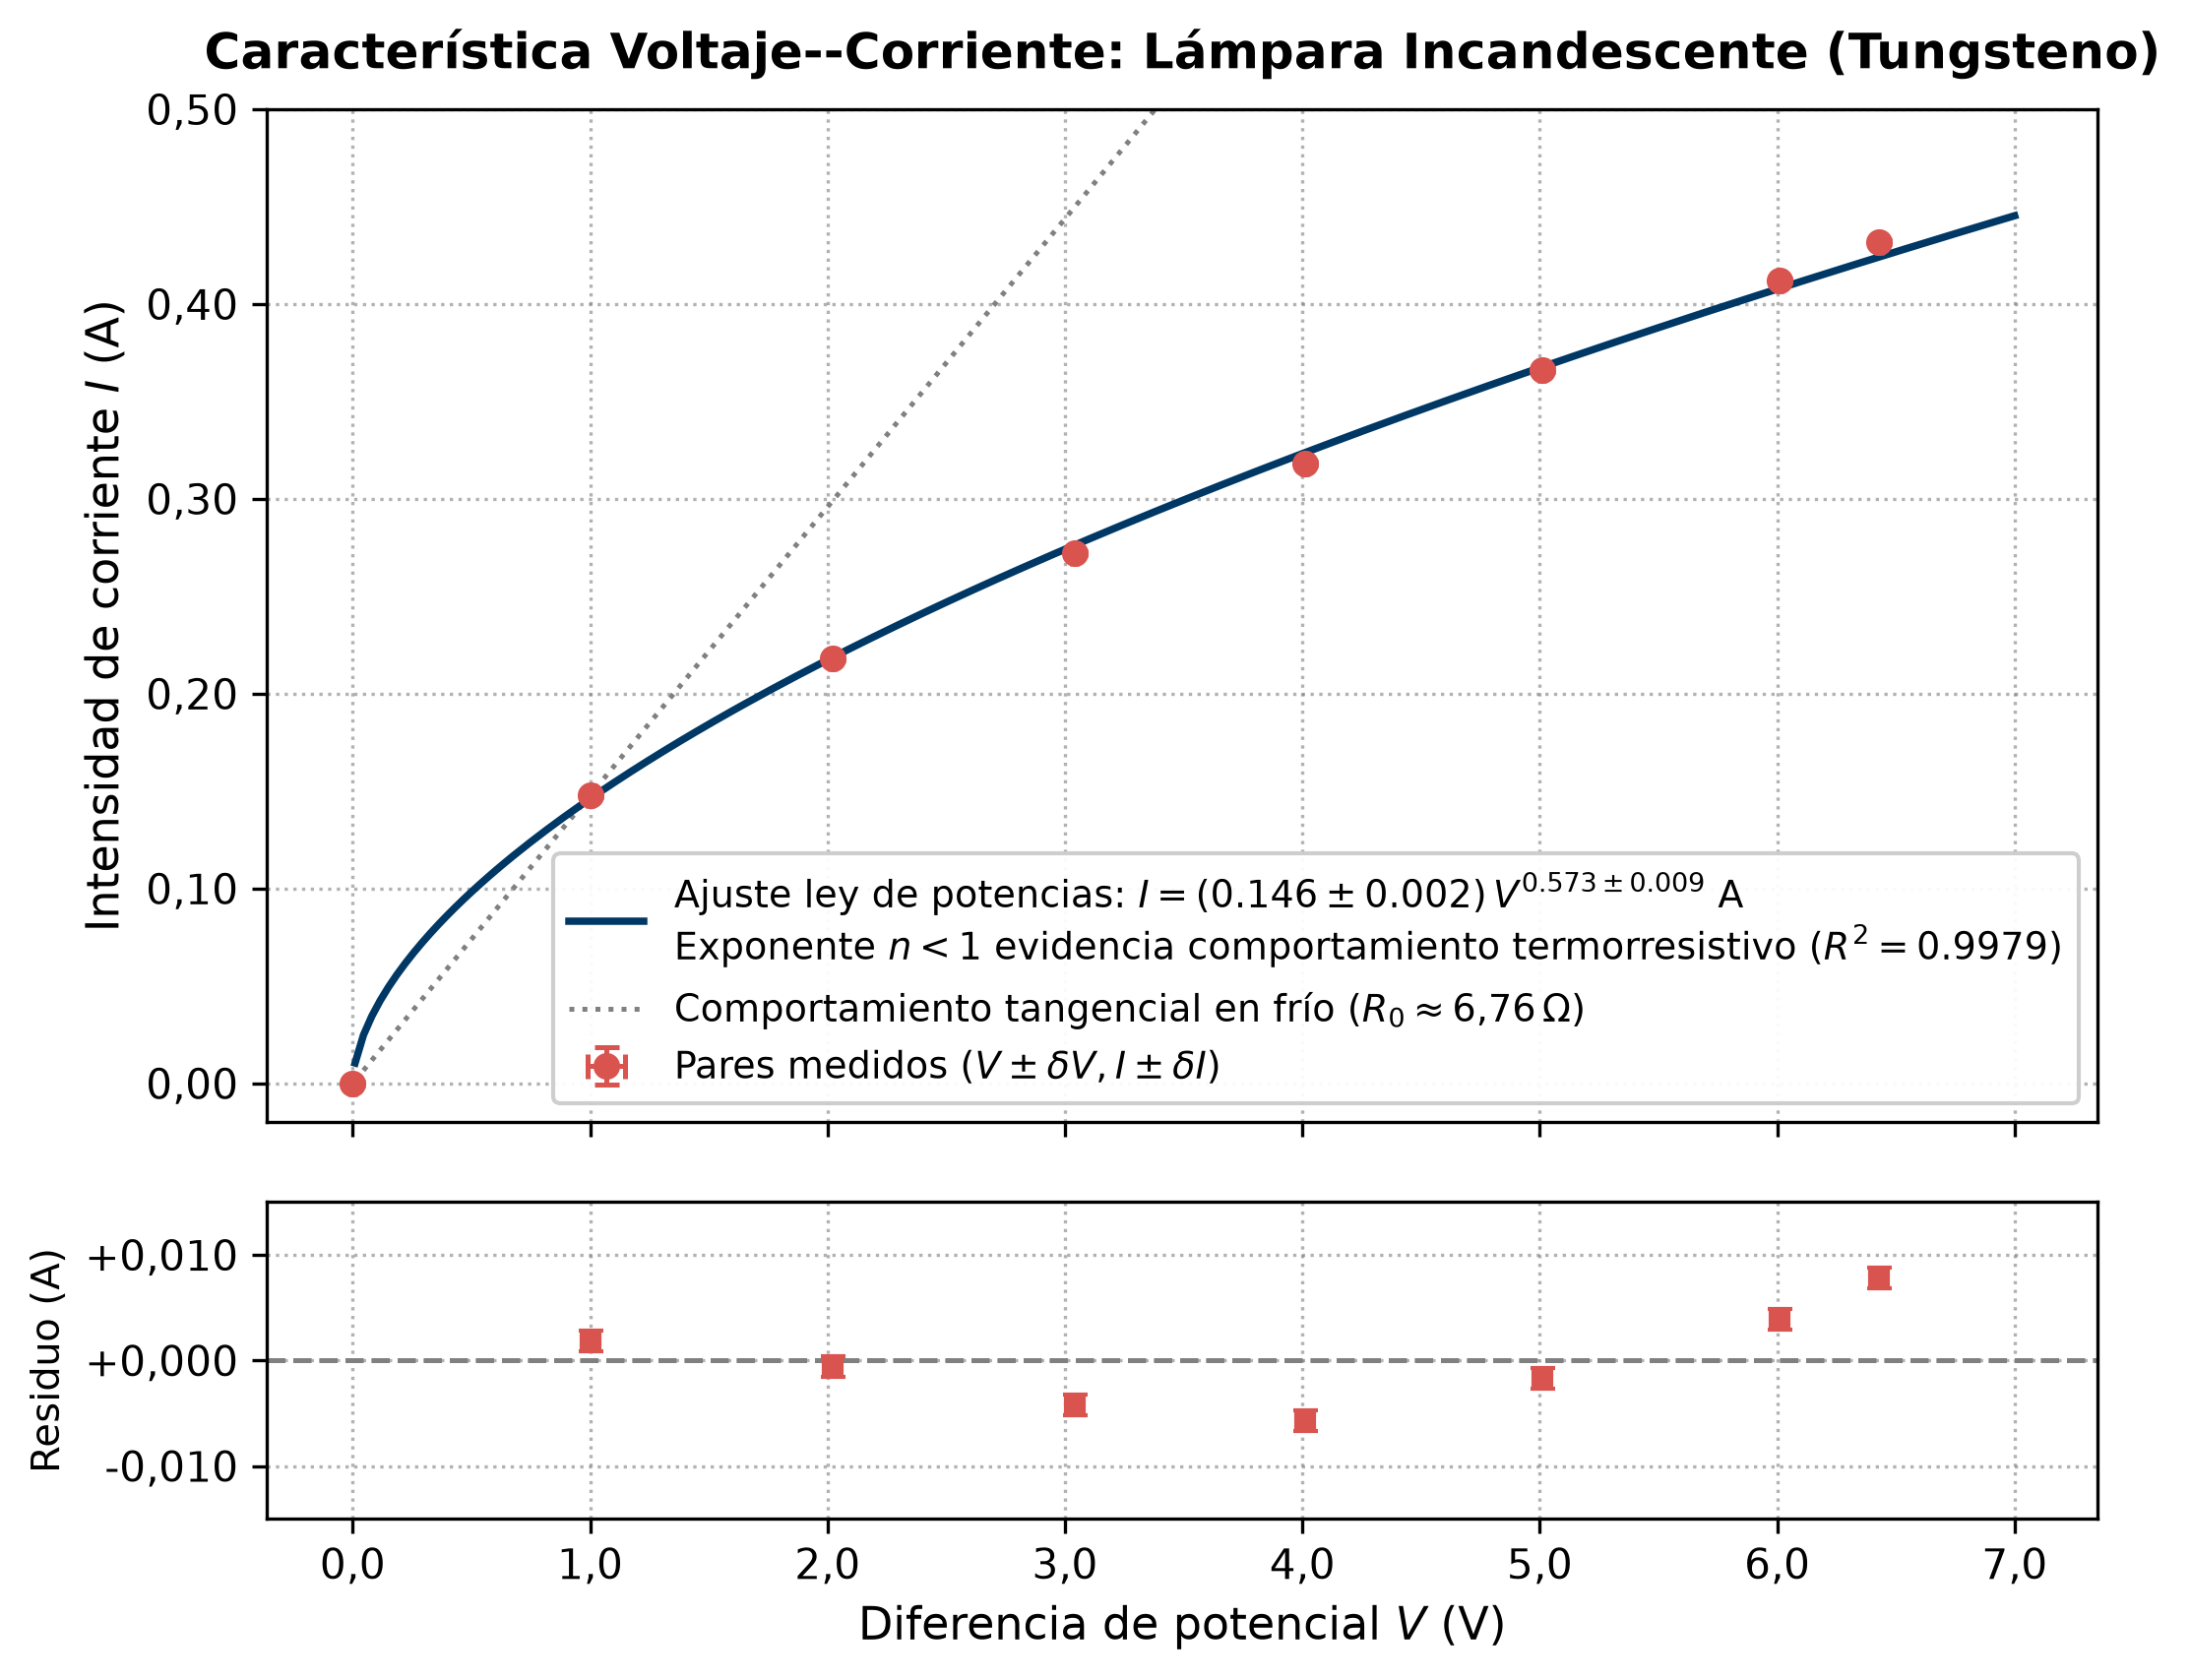
\includegraphics[width=0.85\linewidth]{fig_foquito_tungsteno}
    \caption{Curva característica $I$ vs $V$ de la lámpara incandescente de tungsteno. Los puntos rojos indican los datos experimentales con barras de error. La curva continua azul ilustra el ajuste por ley de potencias $I = (0{,}146 \pm 0{,}003)\,V^{0{,}573 \pm 0{,}014}$ ($R^2 = 0{,}9987$). La recta punteada gris representa el comportamiento tangencial asintótico en frío ($R_0 \approx \qty{6,76}{\ohm}$). El panel inferior detalla los residuos del modelo de radiación. Gráfica generada en Python~\cite{script_graficas}.}
    \label{fig:grafica_foquito_tungsteno}
\end{figure}

\subsection{Curva Característica del Diodo Semiconductor de Silicio}
En la Figura~\ref{fig:grafica_diodo_silicio} se presenta la respuesta no lineal del diodo semiconductor de silicio en polarización directa, exhibiendo el bloqueo previo a \qty{0,6}{\volt}, la conducción exponencial posterior y la determinación gráfica de la tensión de umbral ($V_u$).

\begin{figure}[H]
    \centering
    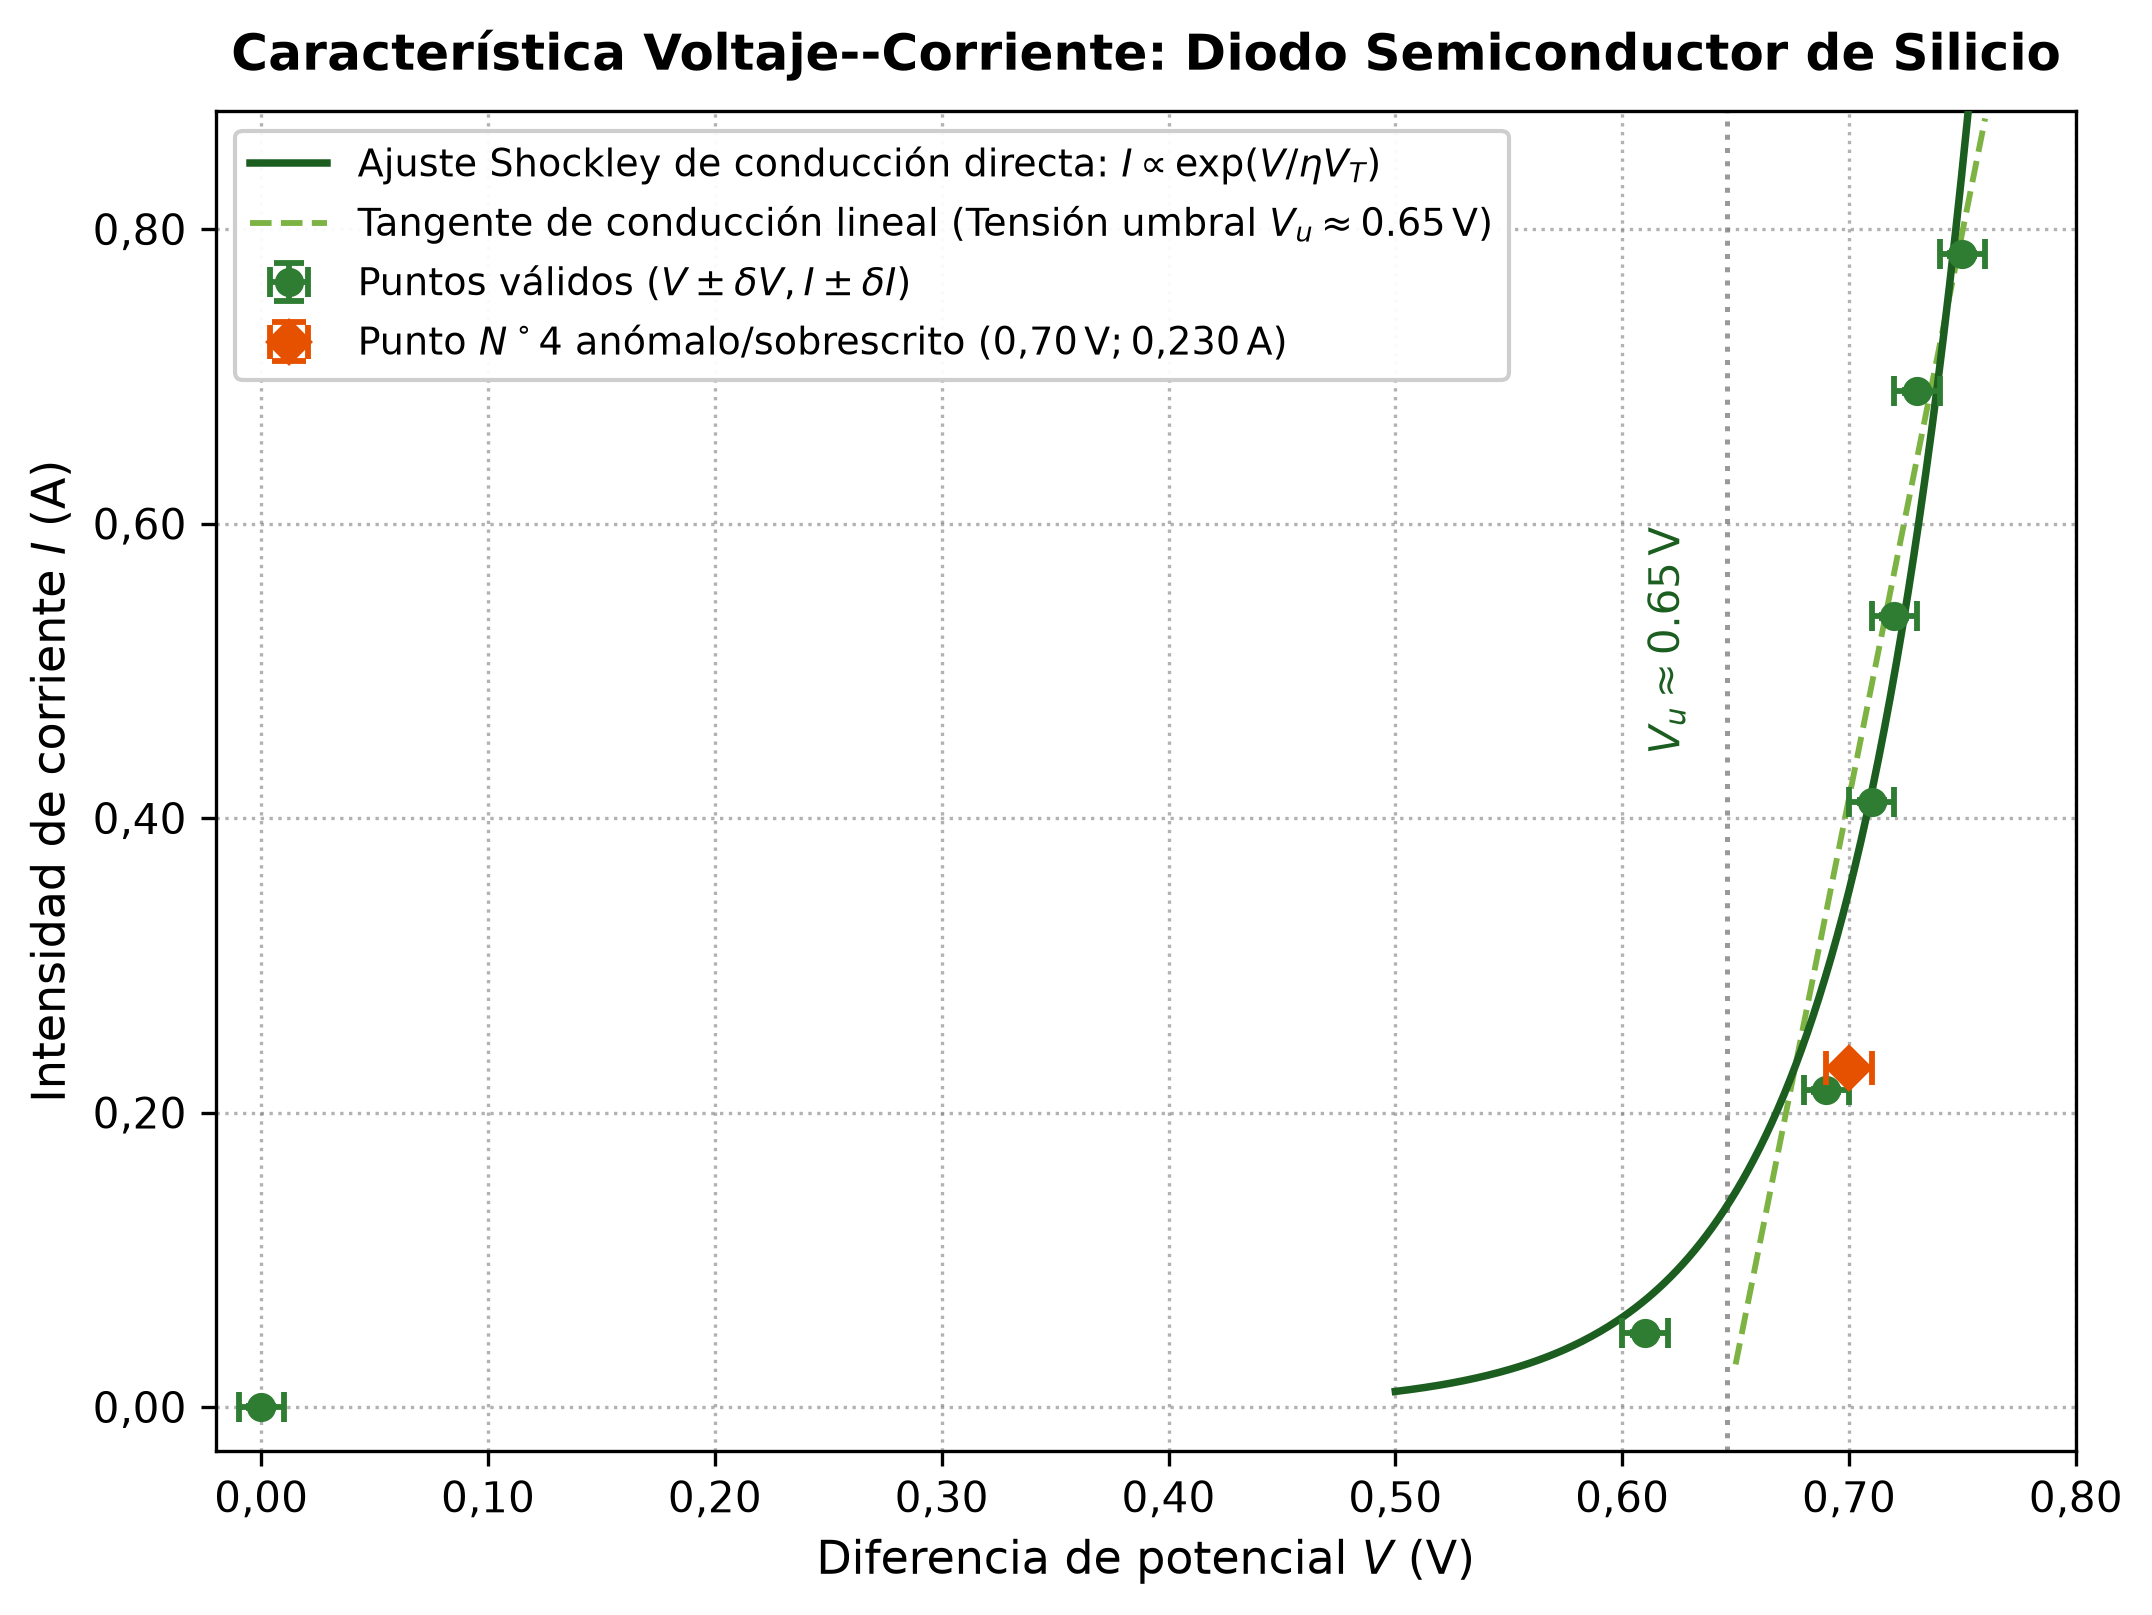
\includegraphics[width=0.85\linewidth]{fig_diodo_silicio}
    \caption{Curva característica $I$ vs $V$ del diodo semiconductor de silicio en polarización directa. Los puntos verdes corresponden a mediciones válidas con barras de error y el rombo naranja destaca el punto atípico $N^\circ 4$ (\qty{0,70}{\volt}; \qty{0,230}{\ampere}). La curva verde continua muestra la tendencia de Shockley y la recta discontinua verde claro representa la tangente de conducción lineal cuya intersección define la tensión de umbral $V_u \approx \qty{0,66}{\volt}$. Gráfica generada en Python~\cite{script_graficas}.}
    \label{fig:grafica_diodo_silicio}
\end{figure}

\subsection{Contraste Comparativo Global de los Tres Elementos}
En la Figura~\ref{fig:grafica_comparativa_elementos} se superponen en una misma escala de potencial y corriente las tres curvas $I$--$V$, permitiendo apreciar de forma inmediata la marcada divergencia entre los regímenes lineal, sublineal y superlineal.

\begin{figure}[H]
    \centering
    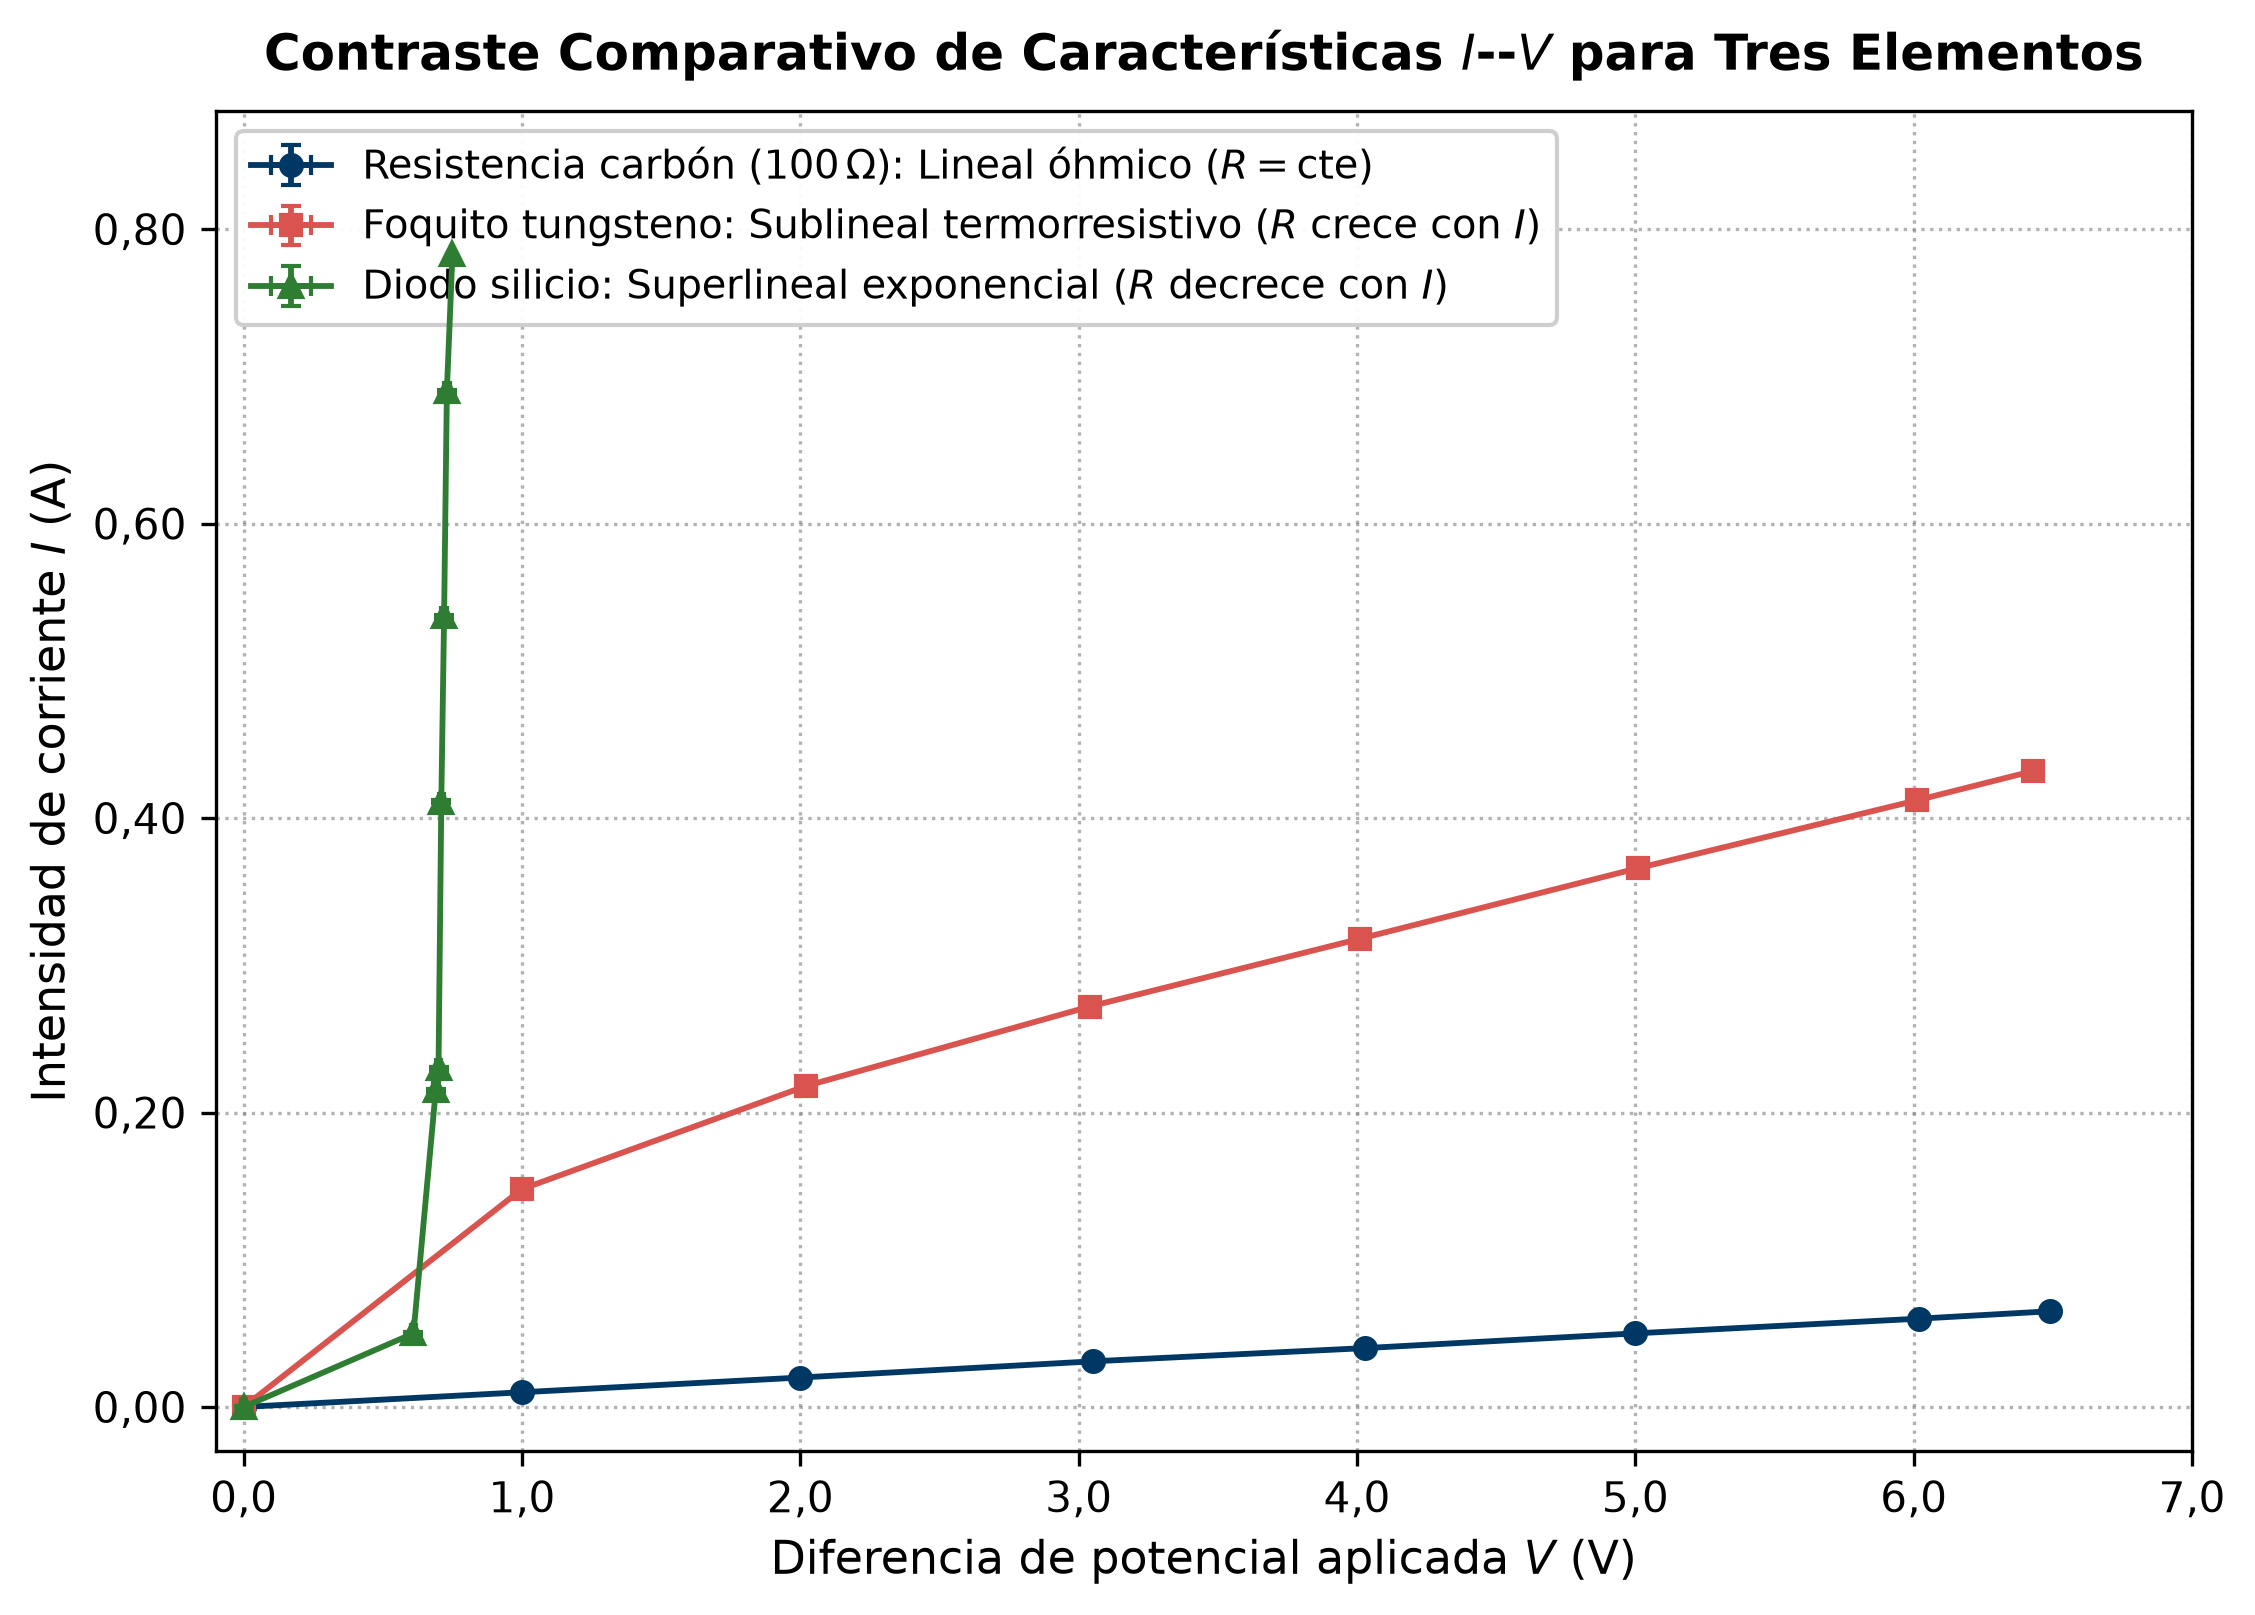
\includegraphics[width=0.85\linewidth]{fig_comparativa_elementos}
    \caption{Contraste comparativo directo de las curvas características $I$--$V$ para la resistencia de carbón (azul, régimen óhmico lineal), lámpara de tungsteno (rojo, régimen sublineal termorresistivo) y diodo de silicio (verde, régimen superlineal exponencial). Se evidencian las diferencias cualitativas y cuantitativas en los órdenes de magnitud de la corriente conducida. Gráfica generada en Python~\cite{script_graficas}.}
    \label{fig:grafica_comparativa_elementos}
\end{figure}

\subsection{Evolución de la Resistencia Estática Aparente \texorpdfstring{$R(I) = V/I$}{R(I) = V/I}}
En la Figura~\ref{fig:grafica_resistencia_vs_corriente} se grafica la resistencia aparente $R = V/I$ en función de la corriente de excitación $I$ para los tres componentes ensayados, ilustrando su comportamiento invariante, monótonamente creciente y monótonamente decreciente.

\begin{figure}[H]
    \centering
    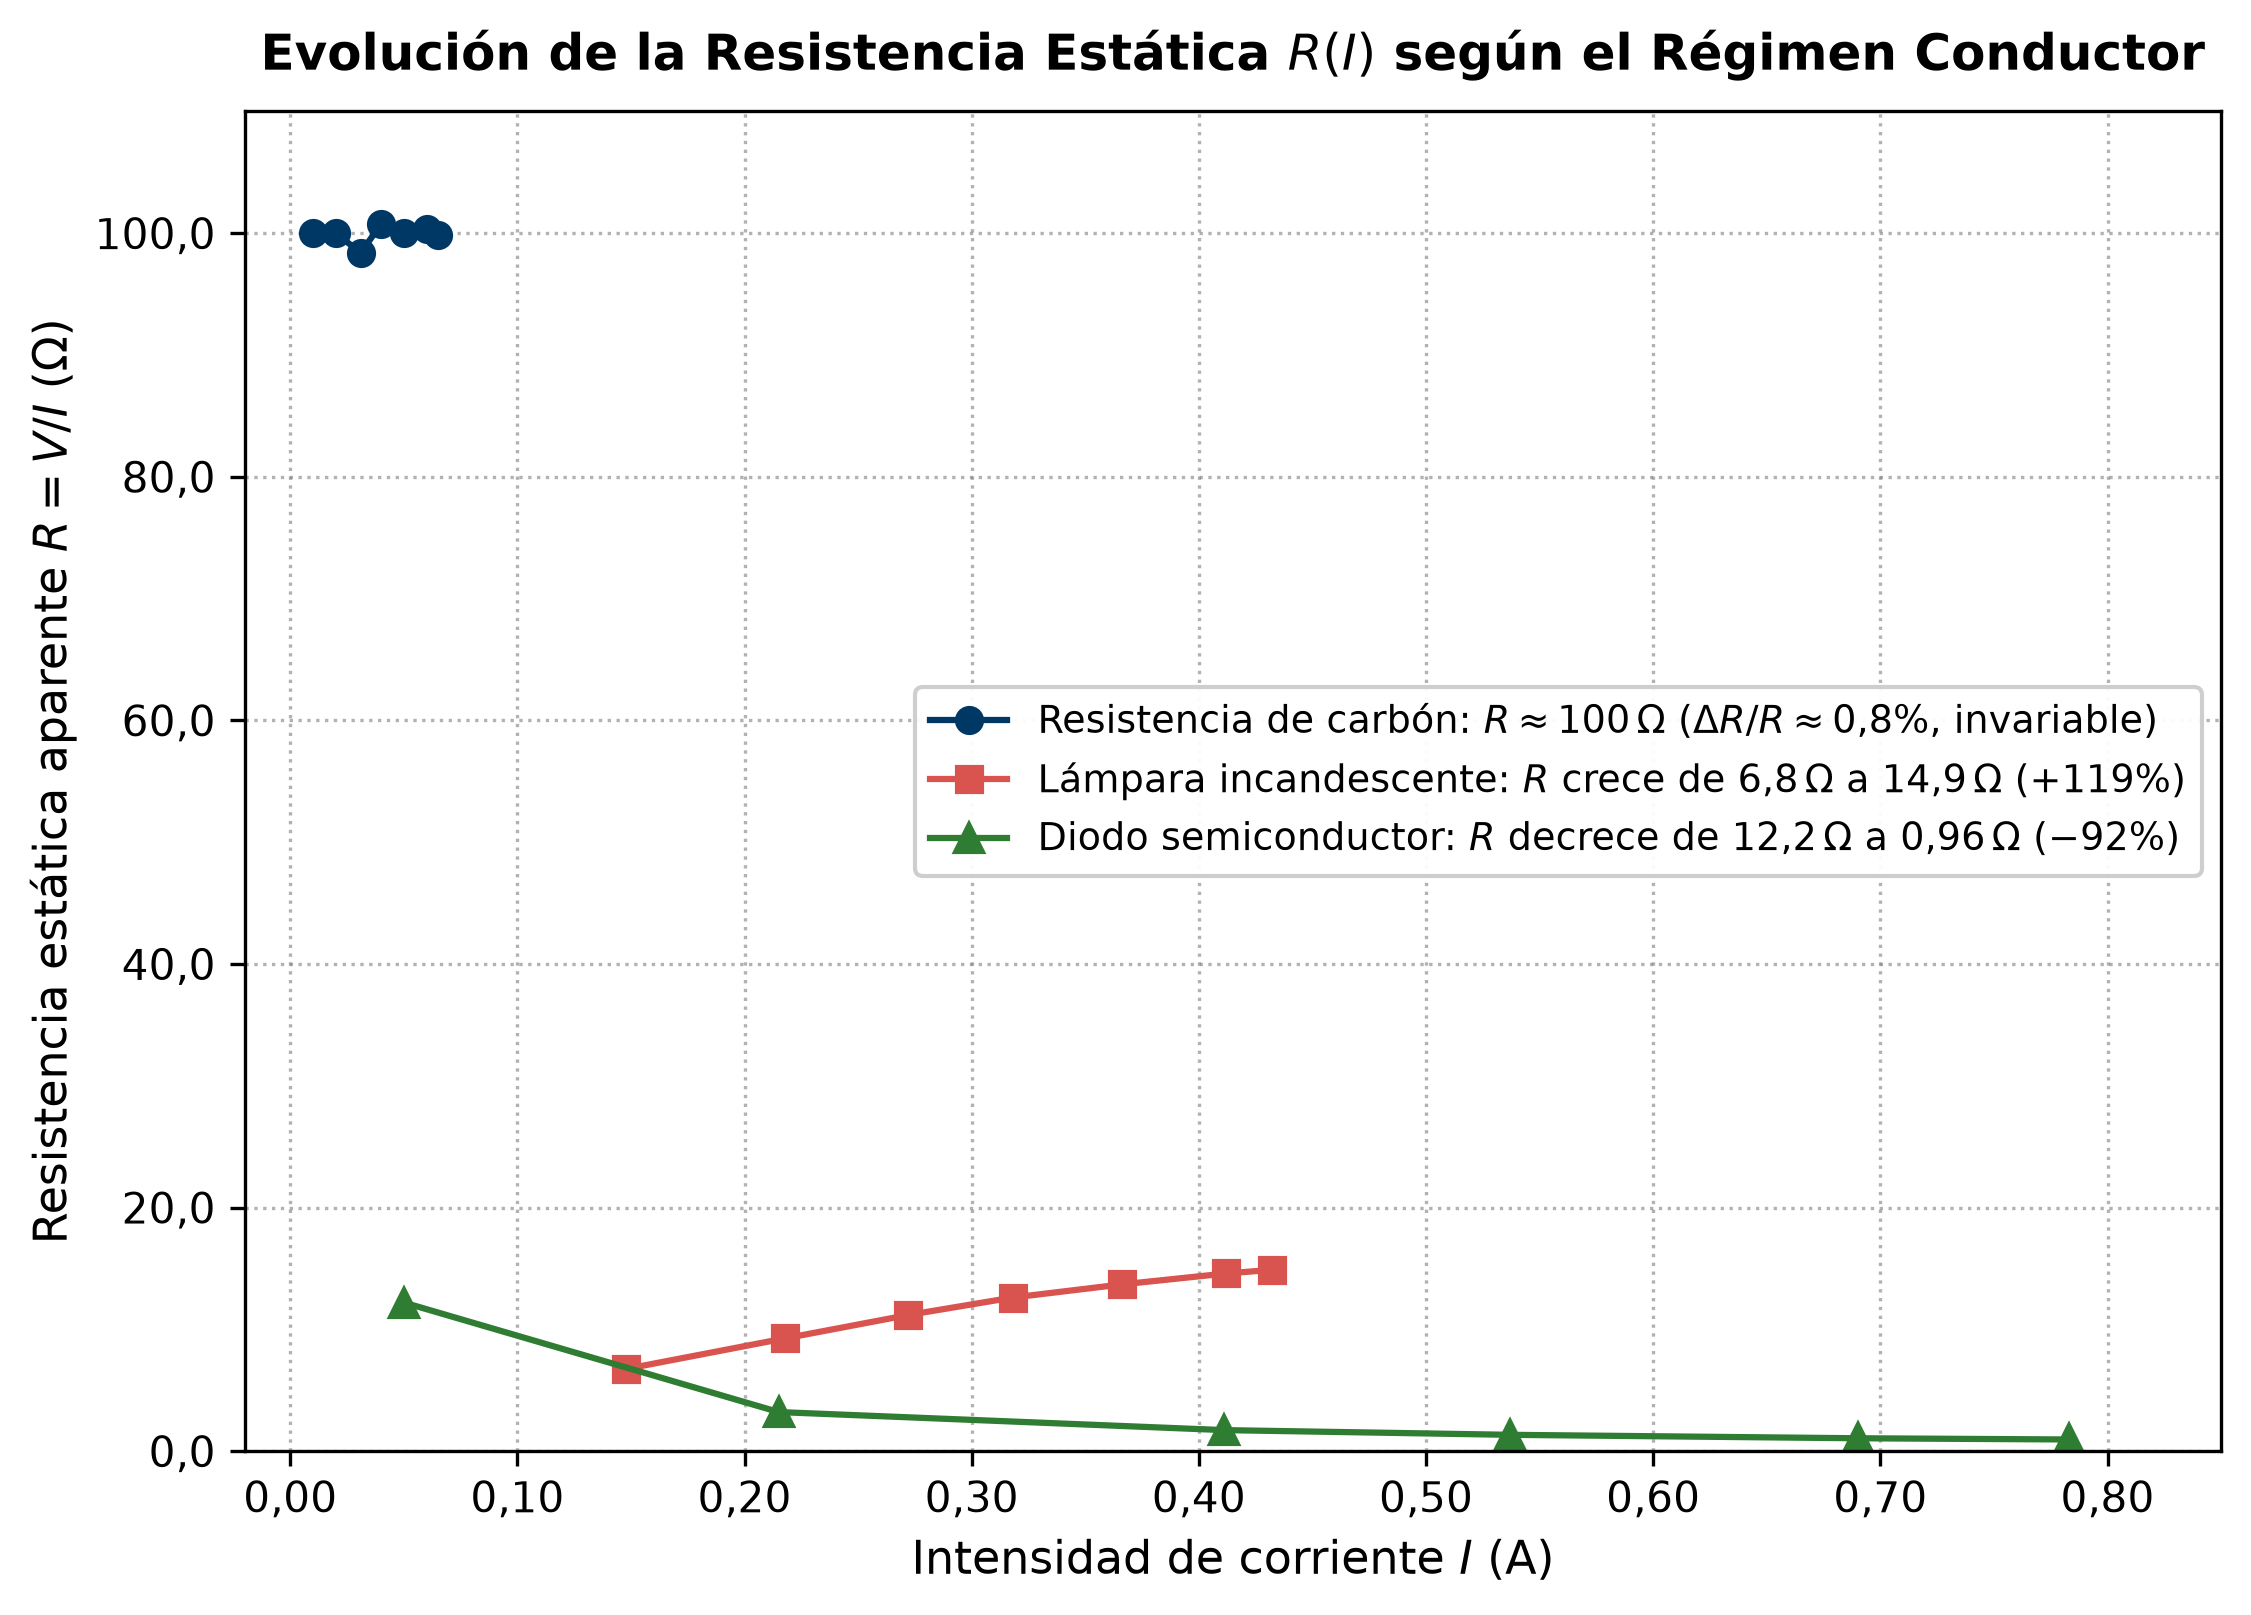
\includegraphics[width=0.85\linewidth]{fig_resistencia_vs_corriente}
    \caption{Evolución de la resistencia estática aparente $R = V/I$ en función de la corriente $I$. Se comprueba la perfecta horizontalidad del resistor de carbón ($R \approx \qty{100}{\ohm}$, variación $< \qty{1}{\percent}$), el crecimiento de la lámpara de \qty{6,8}{\ohm} a \qty{14,9}{\ohm} ($+119\%$) y el colapso del diodo de \qty{12,2}{\ohm} a \qty{0,96}{\ohm} ($-92\%$). Gráfica generada en Python~\cite{script_graficas}.}
    \label{fig:grafica_resistencia_vs_corriente}
\end{figure}

Las curvas científicas expuestas en las Figuras~\ref{fig:grafica_resistencia_ohmica} a~\ref{fig:grafica_resistencia_vs_corriente} proporcionan la base visual y cuantitativa para examinar la dispersión estadística de los residuos, la compatibilidad de los parámetros de ajuste con los modelos teóricos y las propiedades microscópicas de cada régimen de transporte, aspectos que se analizan detalladamente en la Sección~\ref{sec:analisis_graficas}.
